\subsection{Temporal Forecasting}

Producing business-as-usual (BAU) projections from historical data is a fundamental task in environmental data analysis.
We conduct two case studies to compare forecasting methods on datasets with different characteristics.

\subsubsection{Global Plastic Production}

We apply forecasting models to the \texttt{GlobalPlasticsProduction} dataset.
It contains 59 observations, more than the other time series examined in this study.
The observation for 1974 is missing and is handled as described in Section~\ref{sec:models}.
We also compare grid search and random search in terms of tuning runtime and predictive performance.
We use four forecast origins: 1999, 2004, 2009, and 2014. Each test window contains five observations, starting in 2000, 2005, 2010, and 2015, respectively.

% results/rolling_global_forecasting_grid_search/metric_table
\begin{table}[!ht]
	\centering
	\caption{
		\centering Temporal forecasting performance for global plastic production using grid-search tuning for tunable models, averaged first over 16 runs at each origin and then over four forecast origins, with 5 test observations per origin. The \textsuperscript{*} marker denotes the SVR variant with \(\gamma\) tuning enabled.
	}
	\begin{tabular}{@{}lccccc@{}}
		\toprule
		\textbf{Experiment}    & \textbf{MAE}                   & \textbf{RMSE}                  & $\mathbf{R^2}$     & \textbf{WAPE}       & \textbf{sMAPE}      \\
		\midrule
		Naive Persistence & \(3.990 \times 10^{7}\) & \(4.399 \times 10^{7}\) & -5.015 & 12.41\% & 13.07\% \\
		Drift Baseline & \(2.267 \times 10^{7}\) & \(2.568 \times 10^{7}\) & -0.934 & 6.84\% & 6.99\% \\
		Exponential Smoothing & \(1.495 \times 10^{7}\) & \(1.694 \times 10^{7}\) & -0.202 & 4.40\% & 4.42\% \\
		\textbf{Theil--Sen Regression} & \(\mathbf{1.244 \times 10^{7}}\) & \(\mathbf{1.396 \times 10^{7}}\) & \textbf{0.090} & \textbf{3.75\%} & \textbf{3.75\%} \\
		ARIMA Regression & \(1.593 \times 10^{7}\) & \(1.869 \times 10^{7}\) & -0.540 & 4.70\% & 4.71\% \\
		Ridge Regression & \(2.086 \times 10^{7}\) & \(2.176 \times 10^{7}\) & -0.369 & 6.37\% & 6.53\% \\
		GPR & \(1.856 \times 10^{7}\) & \(2.076 \times 10^{7}\) & -0.558 & 5.29\% & 5.37\% \\
		SVR & \(1.930 \times 10^{7}\) & \(2.249 \times 10^{7}\) & -1.900 & 6.06\% & 6.35\% \\
		SVR\textsuperscript{*} & \(1.789 \times 10^{7}\) & \(1.948 \times 10^{7}\) & -0.654 & 6.17\% & 6.38\% \\
		\hline
	\end{tabular}
	\label{tab:global_forecasting_grid_search_metrics}
\end{table}

% results/rolling_global_forecasting_random_search/metric_table
\begin{table}[!ht]
	\centering
	\caption{\centering Temporal forecasting performance for global plastic production using random-search tuning for tunable models, averaged first over 16 runs at each origin and then over four forecast origins, with 5 test observations per origin. The \textsuperscript{*} marker denotes the SVR variant with \(\gamma\) tuning enabled.}
	\begin{tabular}{@{}lccccc@{}}
		\toprule
		\textbf{Experiment}    & \textbf{MAE}                   & \textbf{RMSE}                  & $\mathbf{R^2}$     & \textbf{WAPE}       & \textbf{sMAPE}      \\
		\midrule
		Naive Persistence & \(3.990 \times 10^{7}\) & \(4.399 \times 10^{7}\) & -5.015 & 12.41\% & 13.07\% \\
		Drift Baseline & \(2.267 \times 10^{7}\) & \(2.568 \times 10^{7}\) & -0.934 & 6.84\% & 6.99\% \\
		Exponential Smoothing & \(1.495 \times 10^{7}\) & \(1.694 \times 10^{7}\) & -0.202 & 4.40\% & 4.42\% \\
		\textbf{Theil--Sen Regression} & \(\mathbf{1.244 \times 10^{7}}\) & \(\mathbf{1.396 \times 10^{7}}\) & \textbf{0.090} & \textbf{3.75\%} & \textbf{3.75\%} \\
		ARIMA Regression & \(1.593 \times 10^{7}\) & \(1.869 \times 10^{7}\) & -0.540 & 4.70\% & 4.71\% \\
		Ridge Regression & \(1.541 \times 10^{7}\) & \(1.641 \times 10^{7}\) & 0.048 & 4.90\% & 4.98\% \\
		GPR & \(1.856 \times 10^{7}\) & \(2.076 \times 10^{7}\) & -0.558 & 5.29\% & 5.37\% \\
		SVR & \(2.047 \times 10^{7}\) & \(2.339 \times 10^{7}\) & -2.095 & 6.45\% & 6.74\% \\
		SVR\textsuperscript{*} & \(2.092 \times 10^{7}\) & \(2.259 \times 10^{7}\) & -1.291 & 7.23\% & 7.54\% \\
		\hline
	\end{tabular}
	\label{tab:global_forecasting_random_search_metrics}
\end{table}


Tables~\ref{tab:global_forecasting_grid_search_metrics} and~\ref{tab:global_forecasting_random_search_metrics} show that Theil--Sen regression achieved the lowest mean MAE, RMSE, WAPE, and sMAPE and the highest mean \(R^2\) among the evaluated methods under both tuning settings. Exponential smoothing achieves the second-lowest WAPE (\(4.40\%\)), followed by ARIMA regression (\(4.70\%\)).
These results summarize the four forecast origins.
Appendix~\ref{sec:appendix_d} reports run-to-run standard deviations calculated within each origin and averaged across origins; they do not represent variability across independent forecast periods.

% results/rolling_global_forecasting_random_search/origin_comparison_table
\begin{table}[!ht]
	\centering
	\caption{WAPE by forecast period for global plastic production. Values are averaged over 16 runs at each origin, using random-search tuning for ridge regression and SVR. The final row gives the equally weighted mean across the four origins.}
	\small
	\begin{tabular}{lrrrr}
		\toprule
		Test years & \shortstack{Exponential\\Smoothing} & \shortstack{Theil--Sen\\Regression} & \shortstack{Ridge\\Regression} & SVR \\
		\midrule
		2000--2004 & 1.00\% & 1.03\% & 7.04\% & 3.70\% \\
		2005--2009 & 3.90\% & 3.63\% & 4.08\% & 4.61\% \\
		2010--2014 & 8.44\% & 7.68\% & 2.27\% & 16.17\% \\
		2015--2019 & 4.25\% & 2.64\% & 6.22\% & 1.31\% \\
		\midrule
		Average across origins & 4.40\% & 3.75\% & 4.90\% & 6.45\% \\
		\bottomrule
	\end{tabular}
	\label{tab:global_forecasting_by_origin}
\end{table}


To examine performance across forecast windows, we report WAPE for exponential smoothing, Theil--Sen regression, ridge regression, and SVR in Table~\ref{tab:global_forecasting_by_origin}.
WAPE is higher in the 2010--2014 window for exponential smoothing, Theil--Sen regression, and SVR than in the other windows.
This increase may be related to the dip in the observed series in 2009, after a generally rising trend.
It is largest for SVR, whose WAPE in that window is \(16.17\%\), compared with \(1.31\%\) in the 2015--2019 window.

\begin{figure}[H]
	\centering
	\subfloat[Theil--Sen regression.]{
		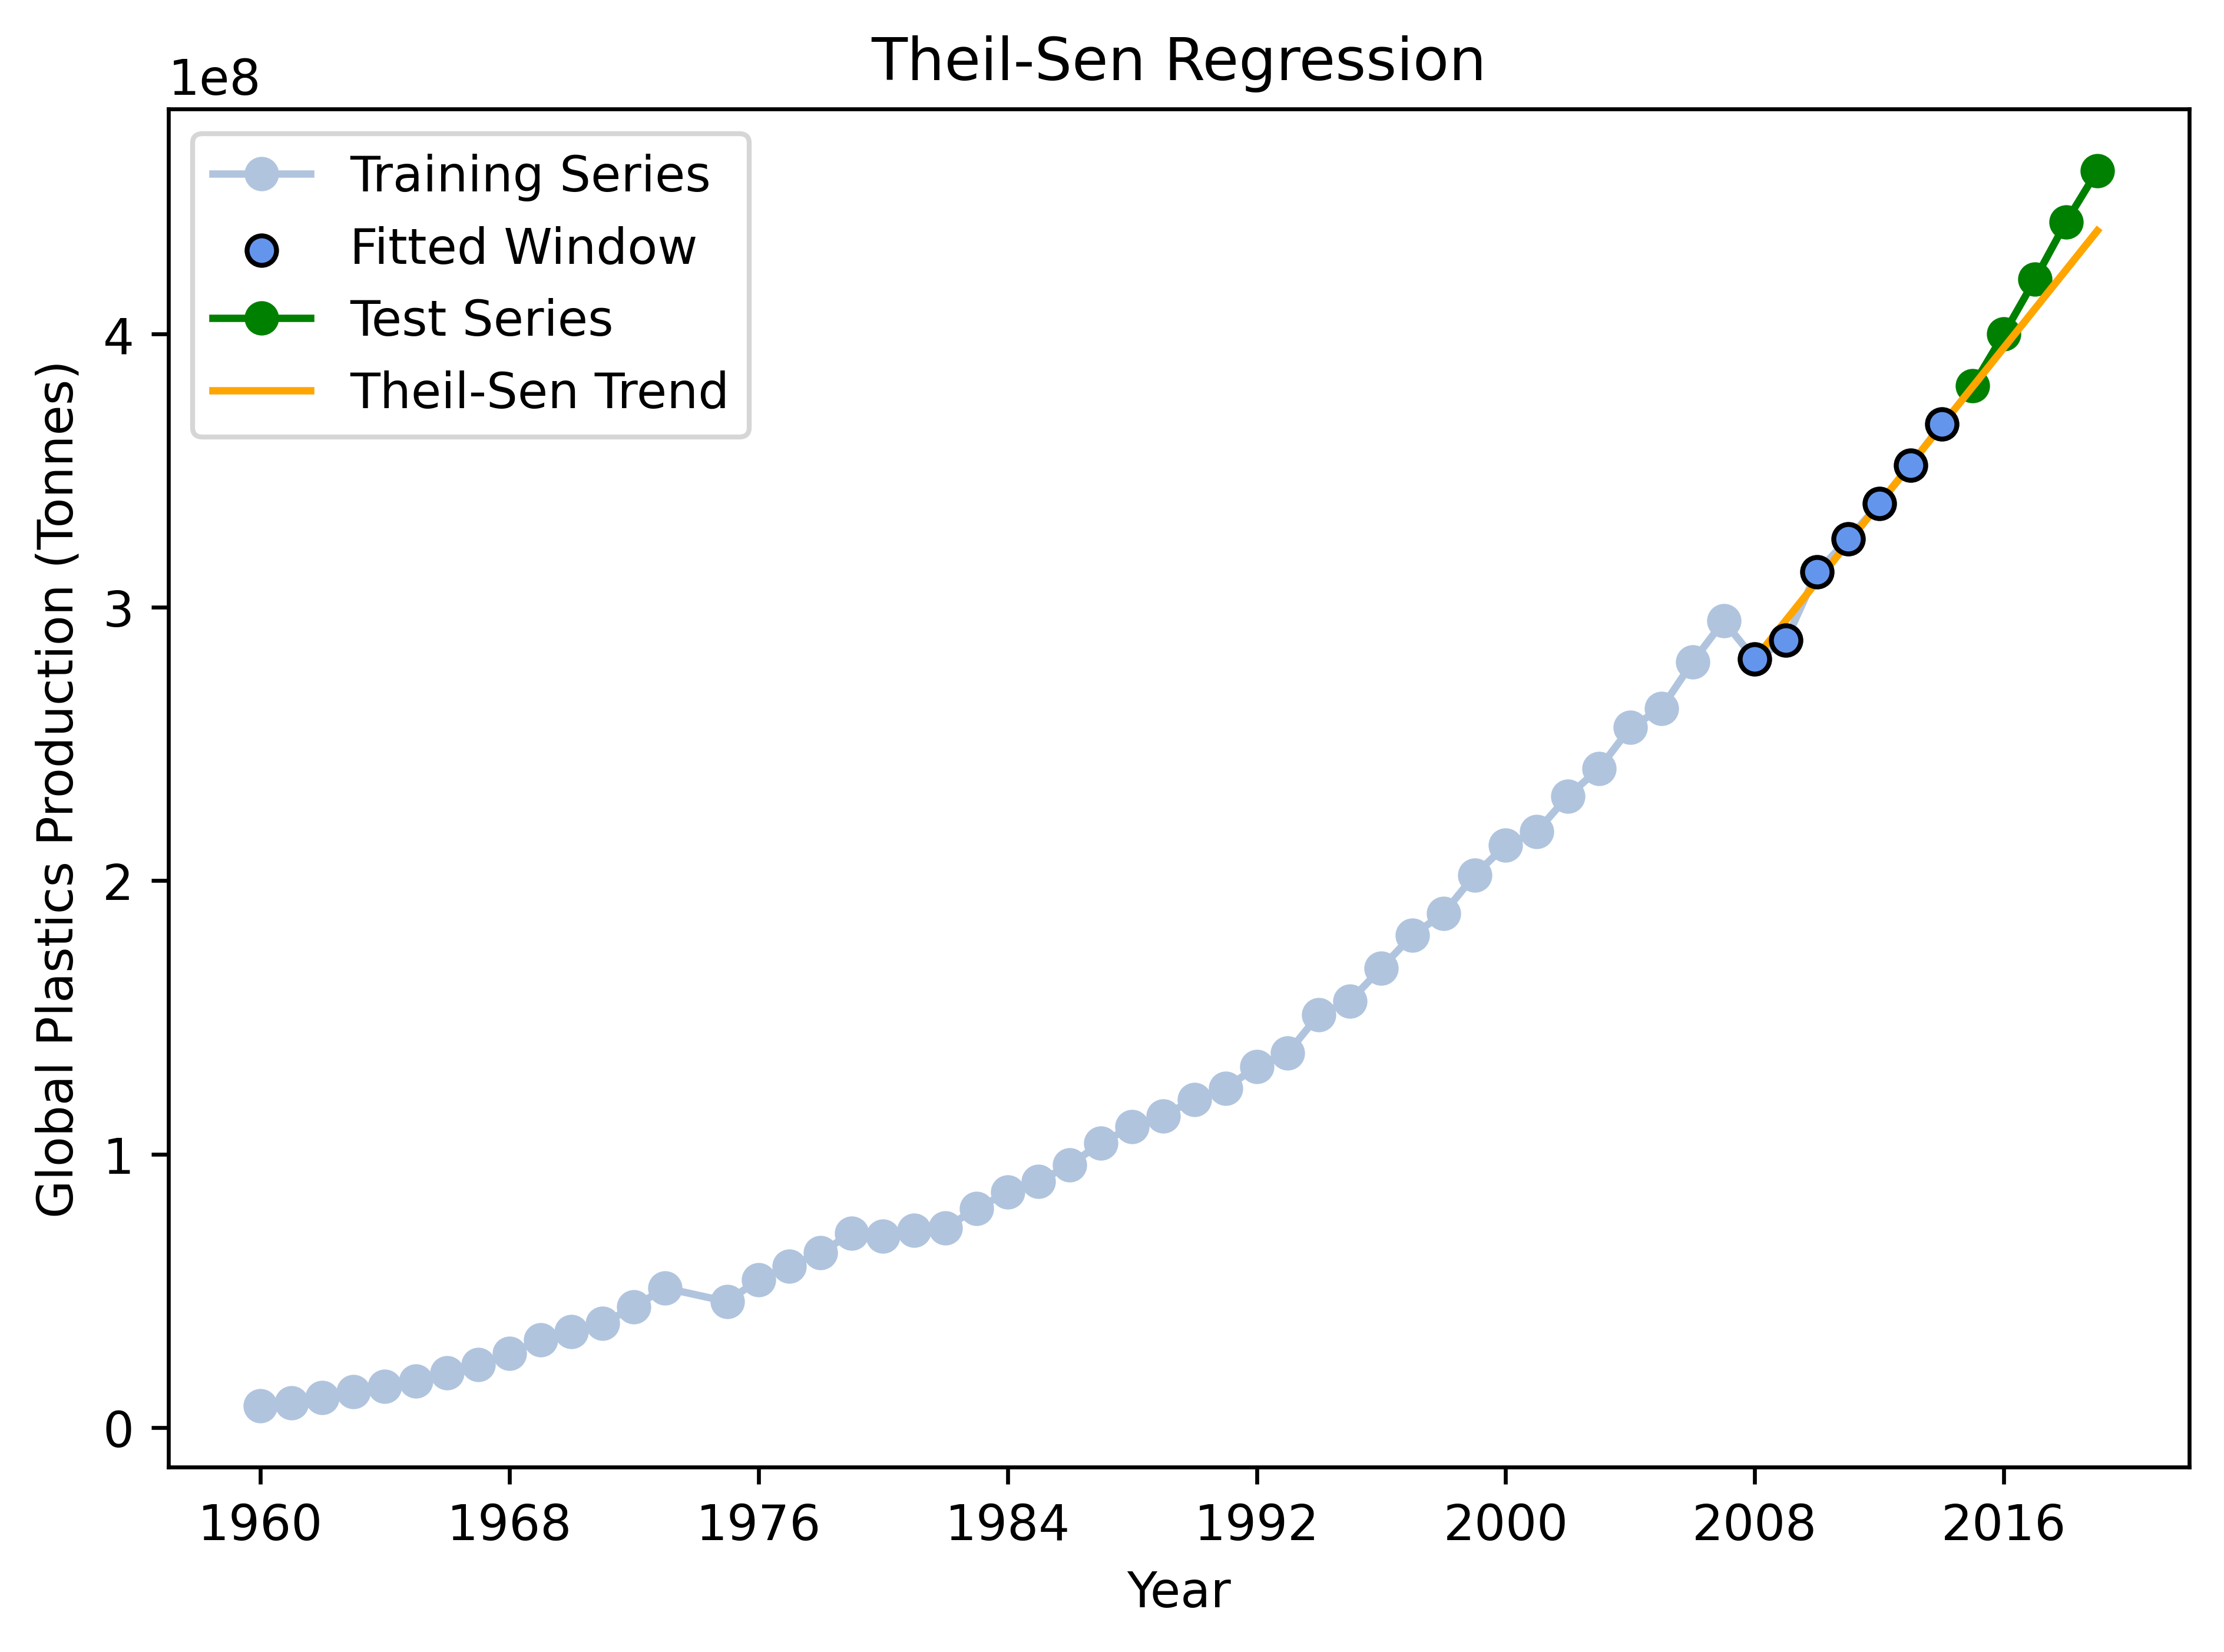
\includegraphics[width=0.45\textwidth]{figures/global_forecasting_theil_sen_regression.png}
	}
	\hfill
	\subfloat[Ridge regression.]{
		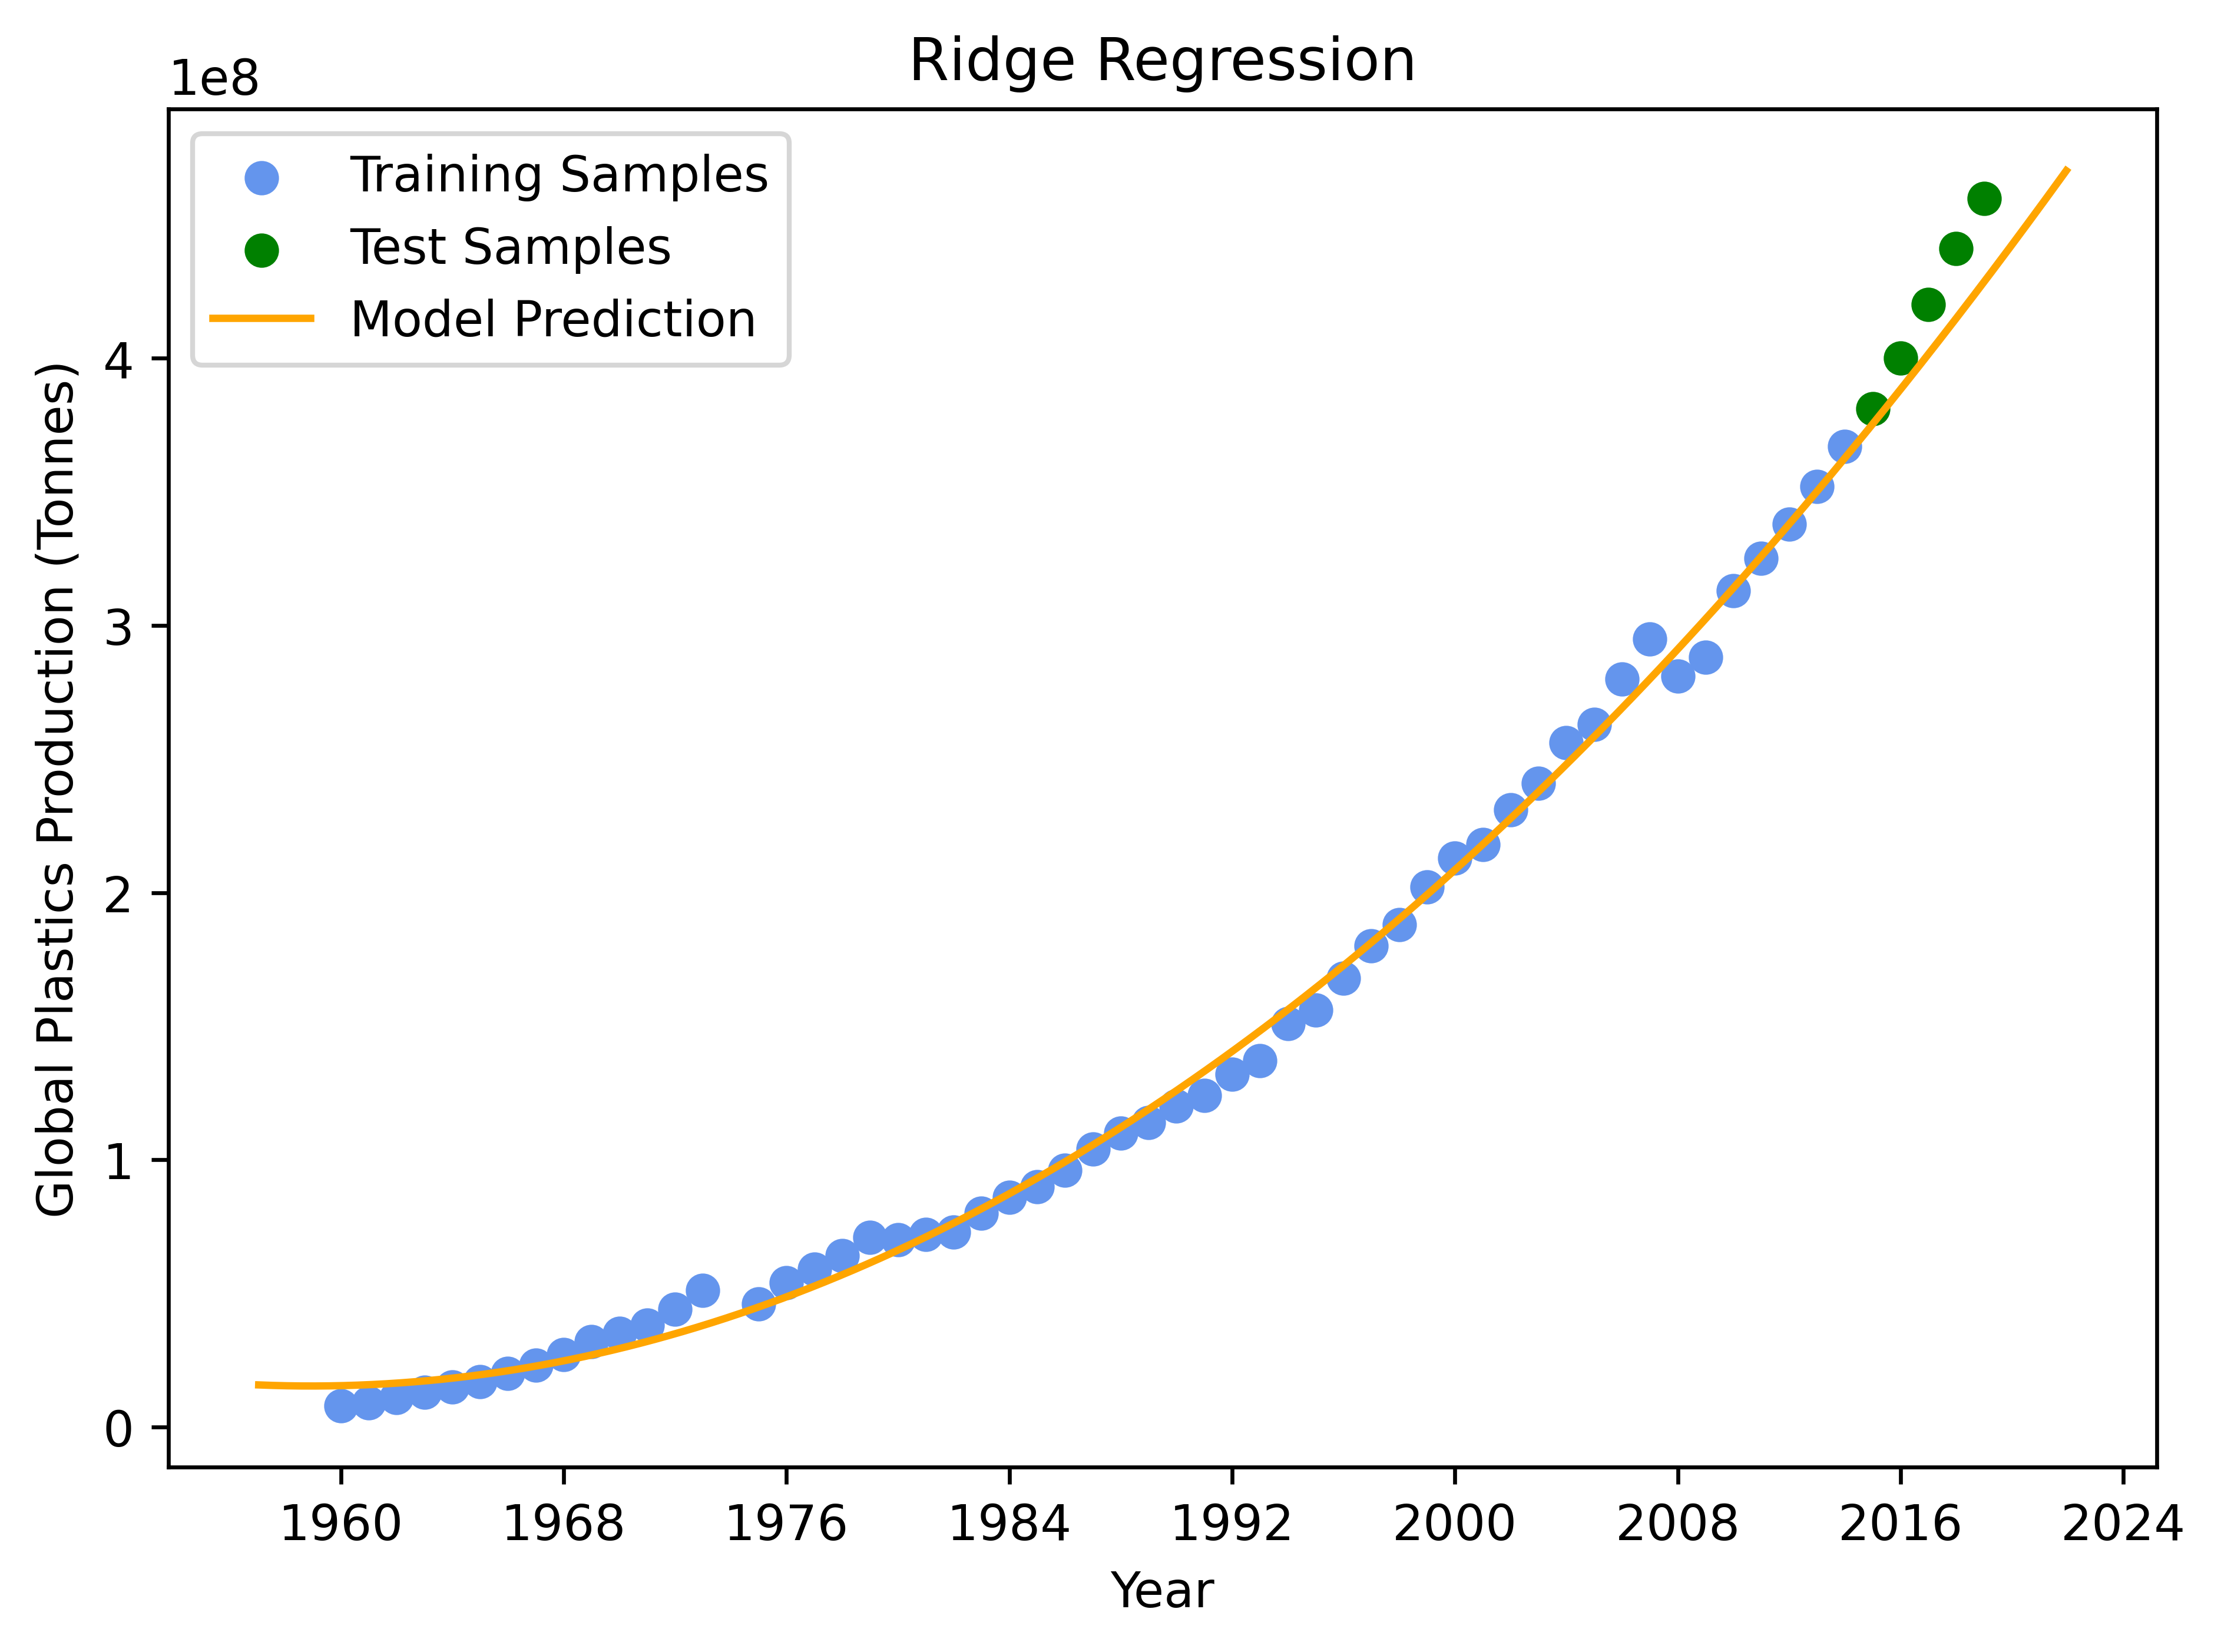
\includegraphics[width=0.45\textwidth]{figures/global_forecasting_ridge_regression.png}
	}

	\vspace{0.5cm}

	\subfloat[GPR.]{
		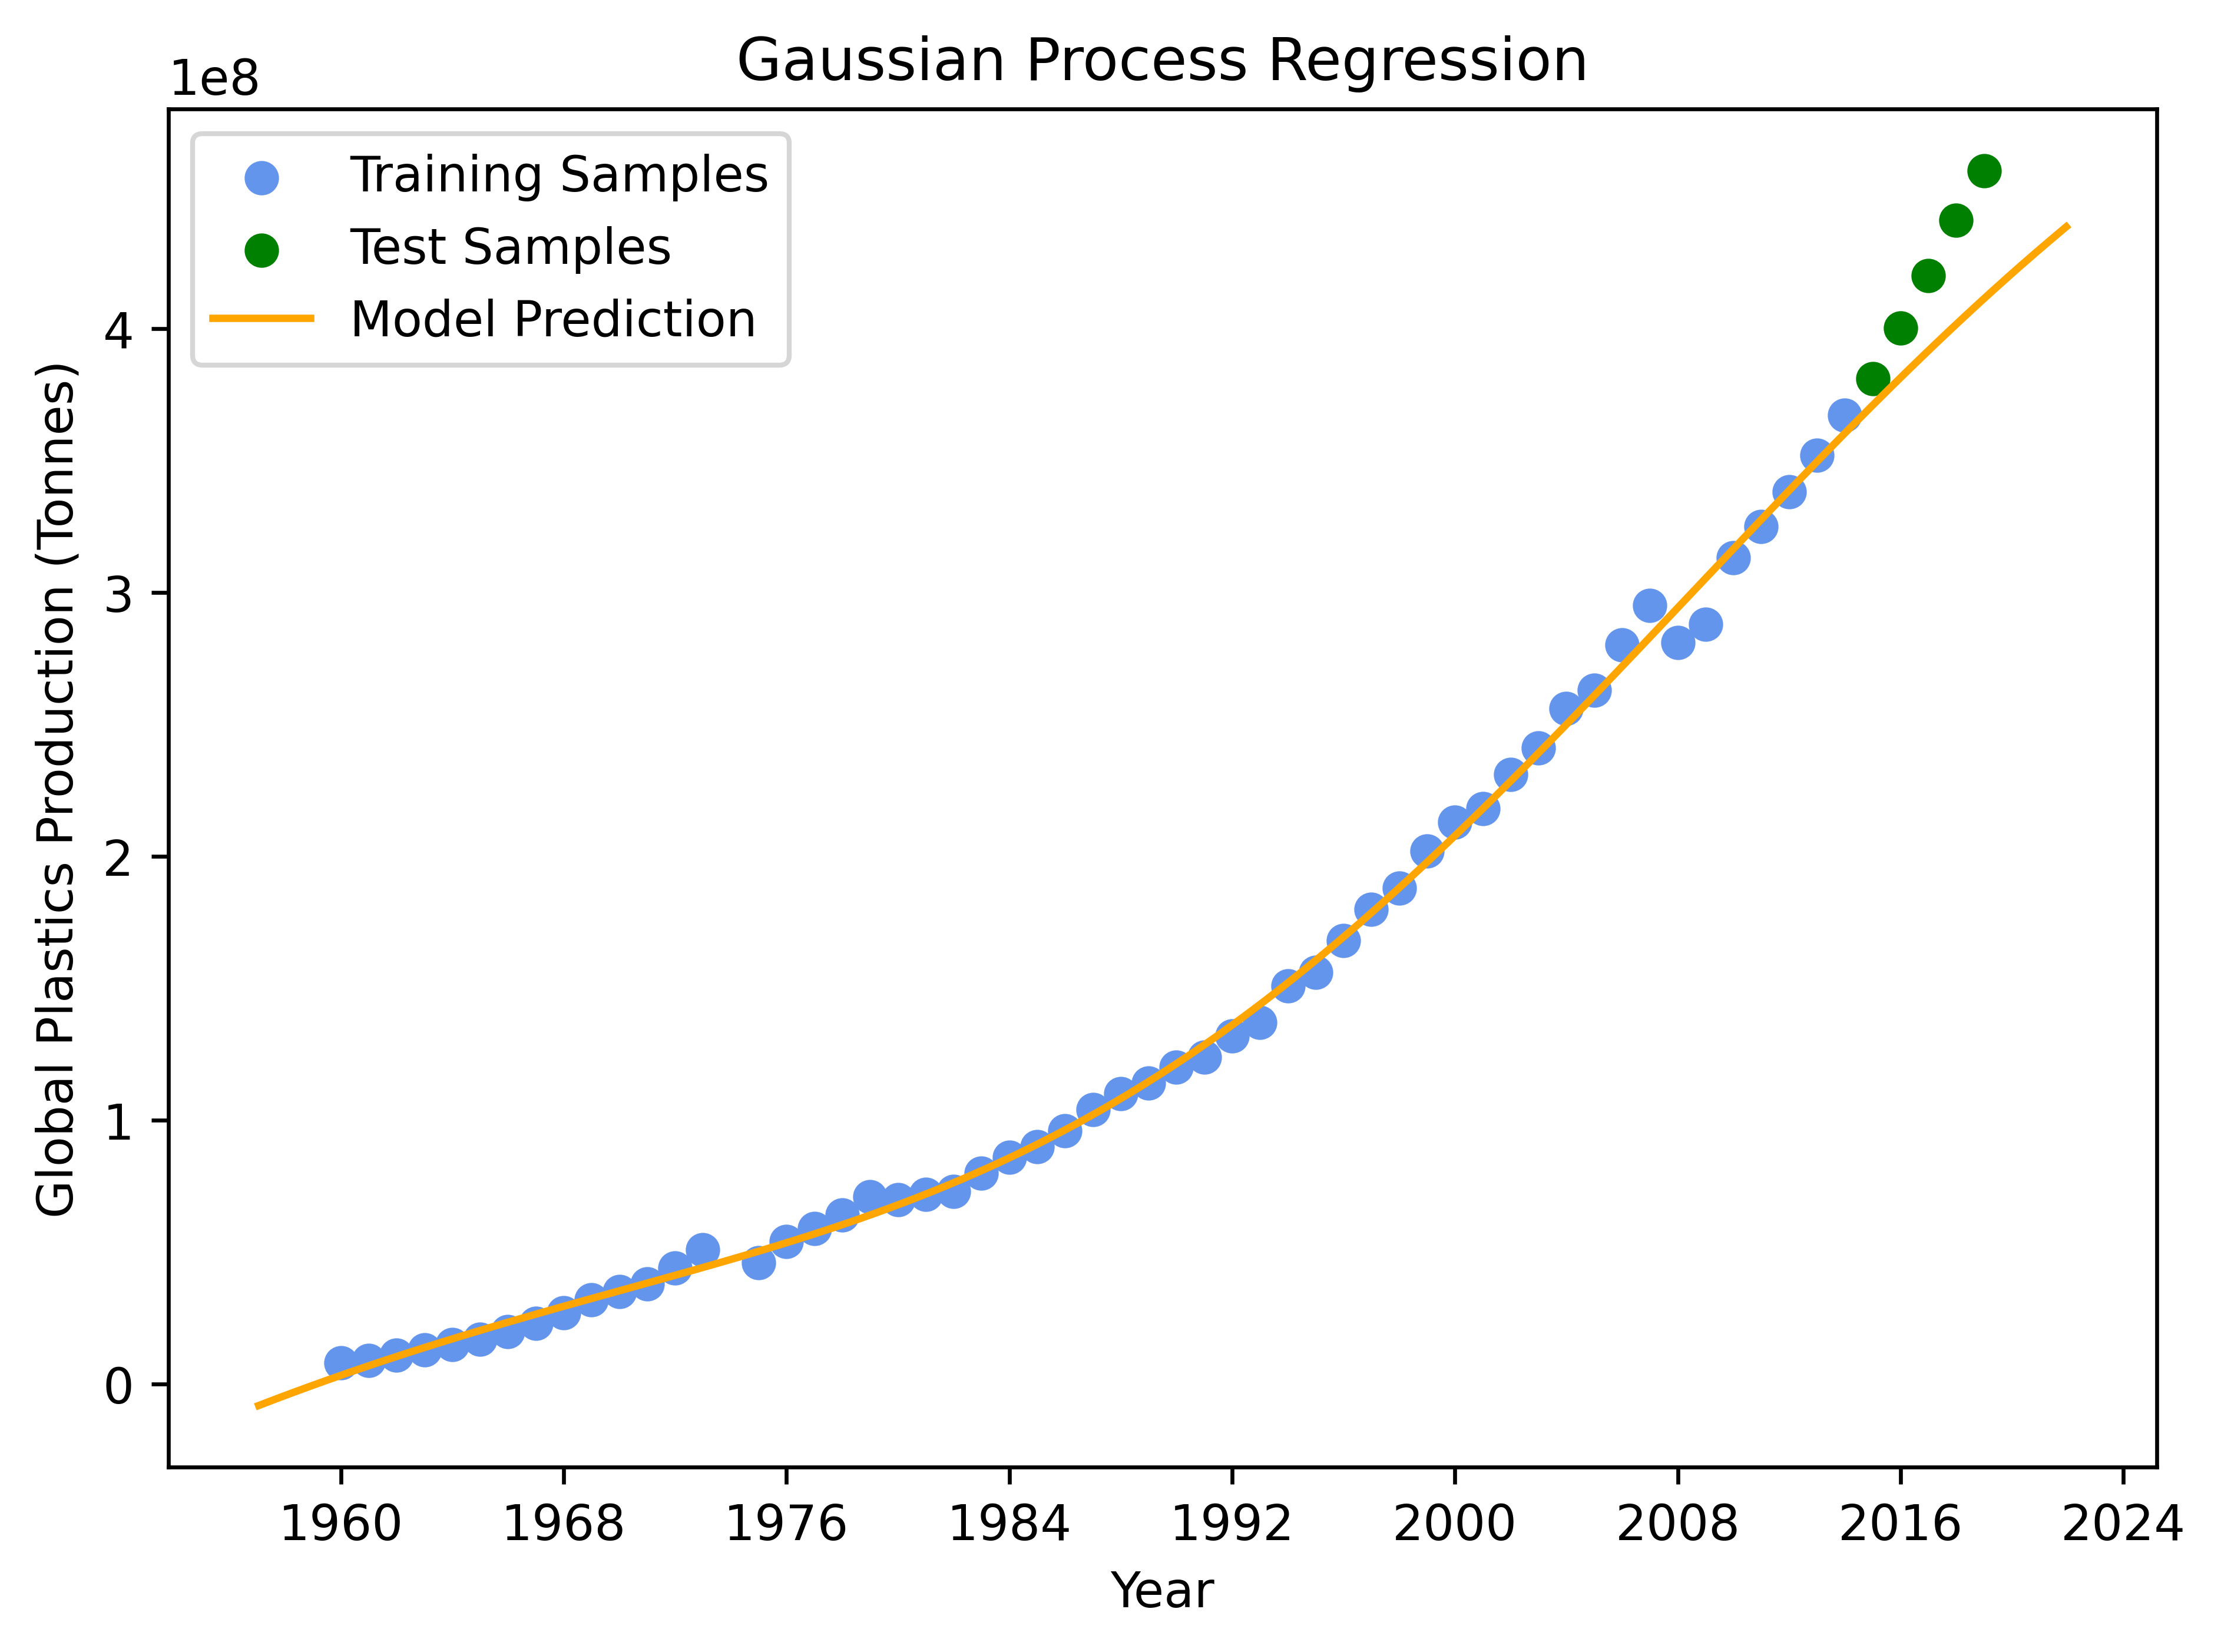
\includegraphics[width=0.45\textwidth]{figures/global_forecasting_gpr.png}
	}
	\subfloat[SVR.]{
		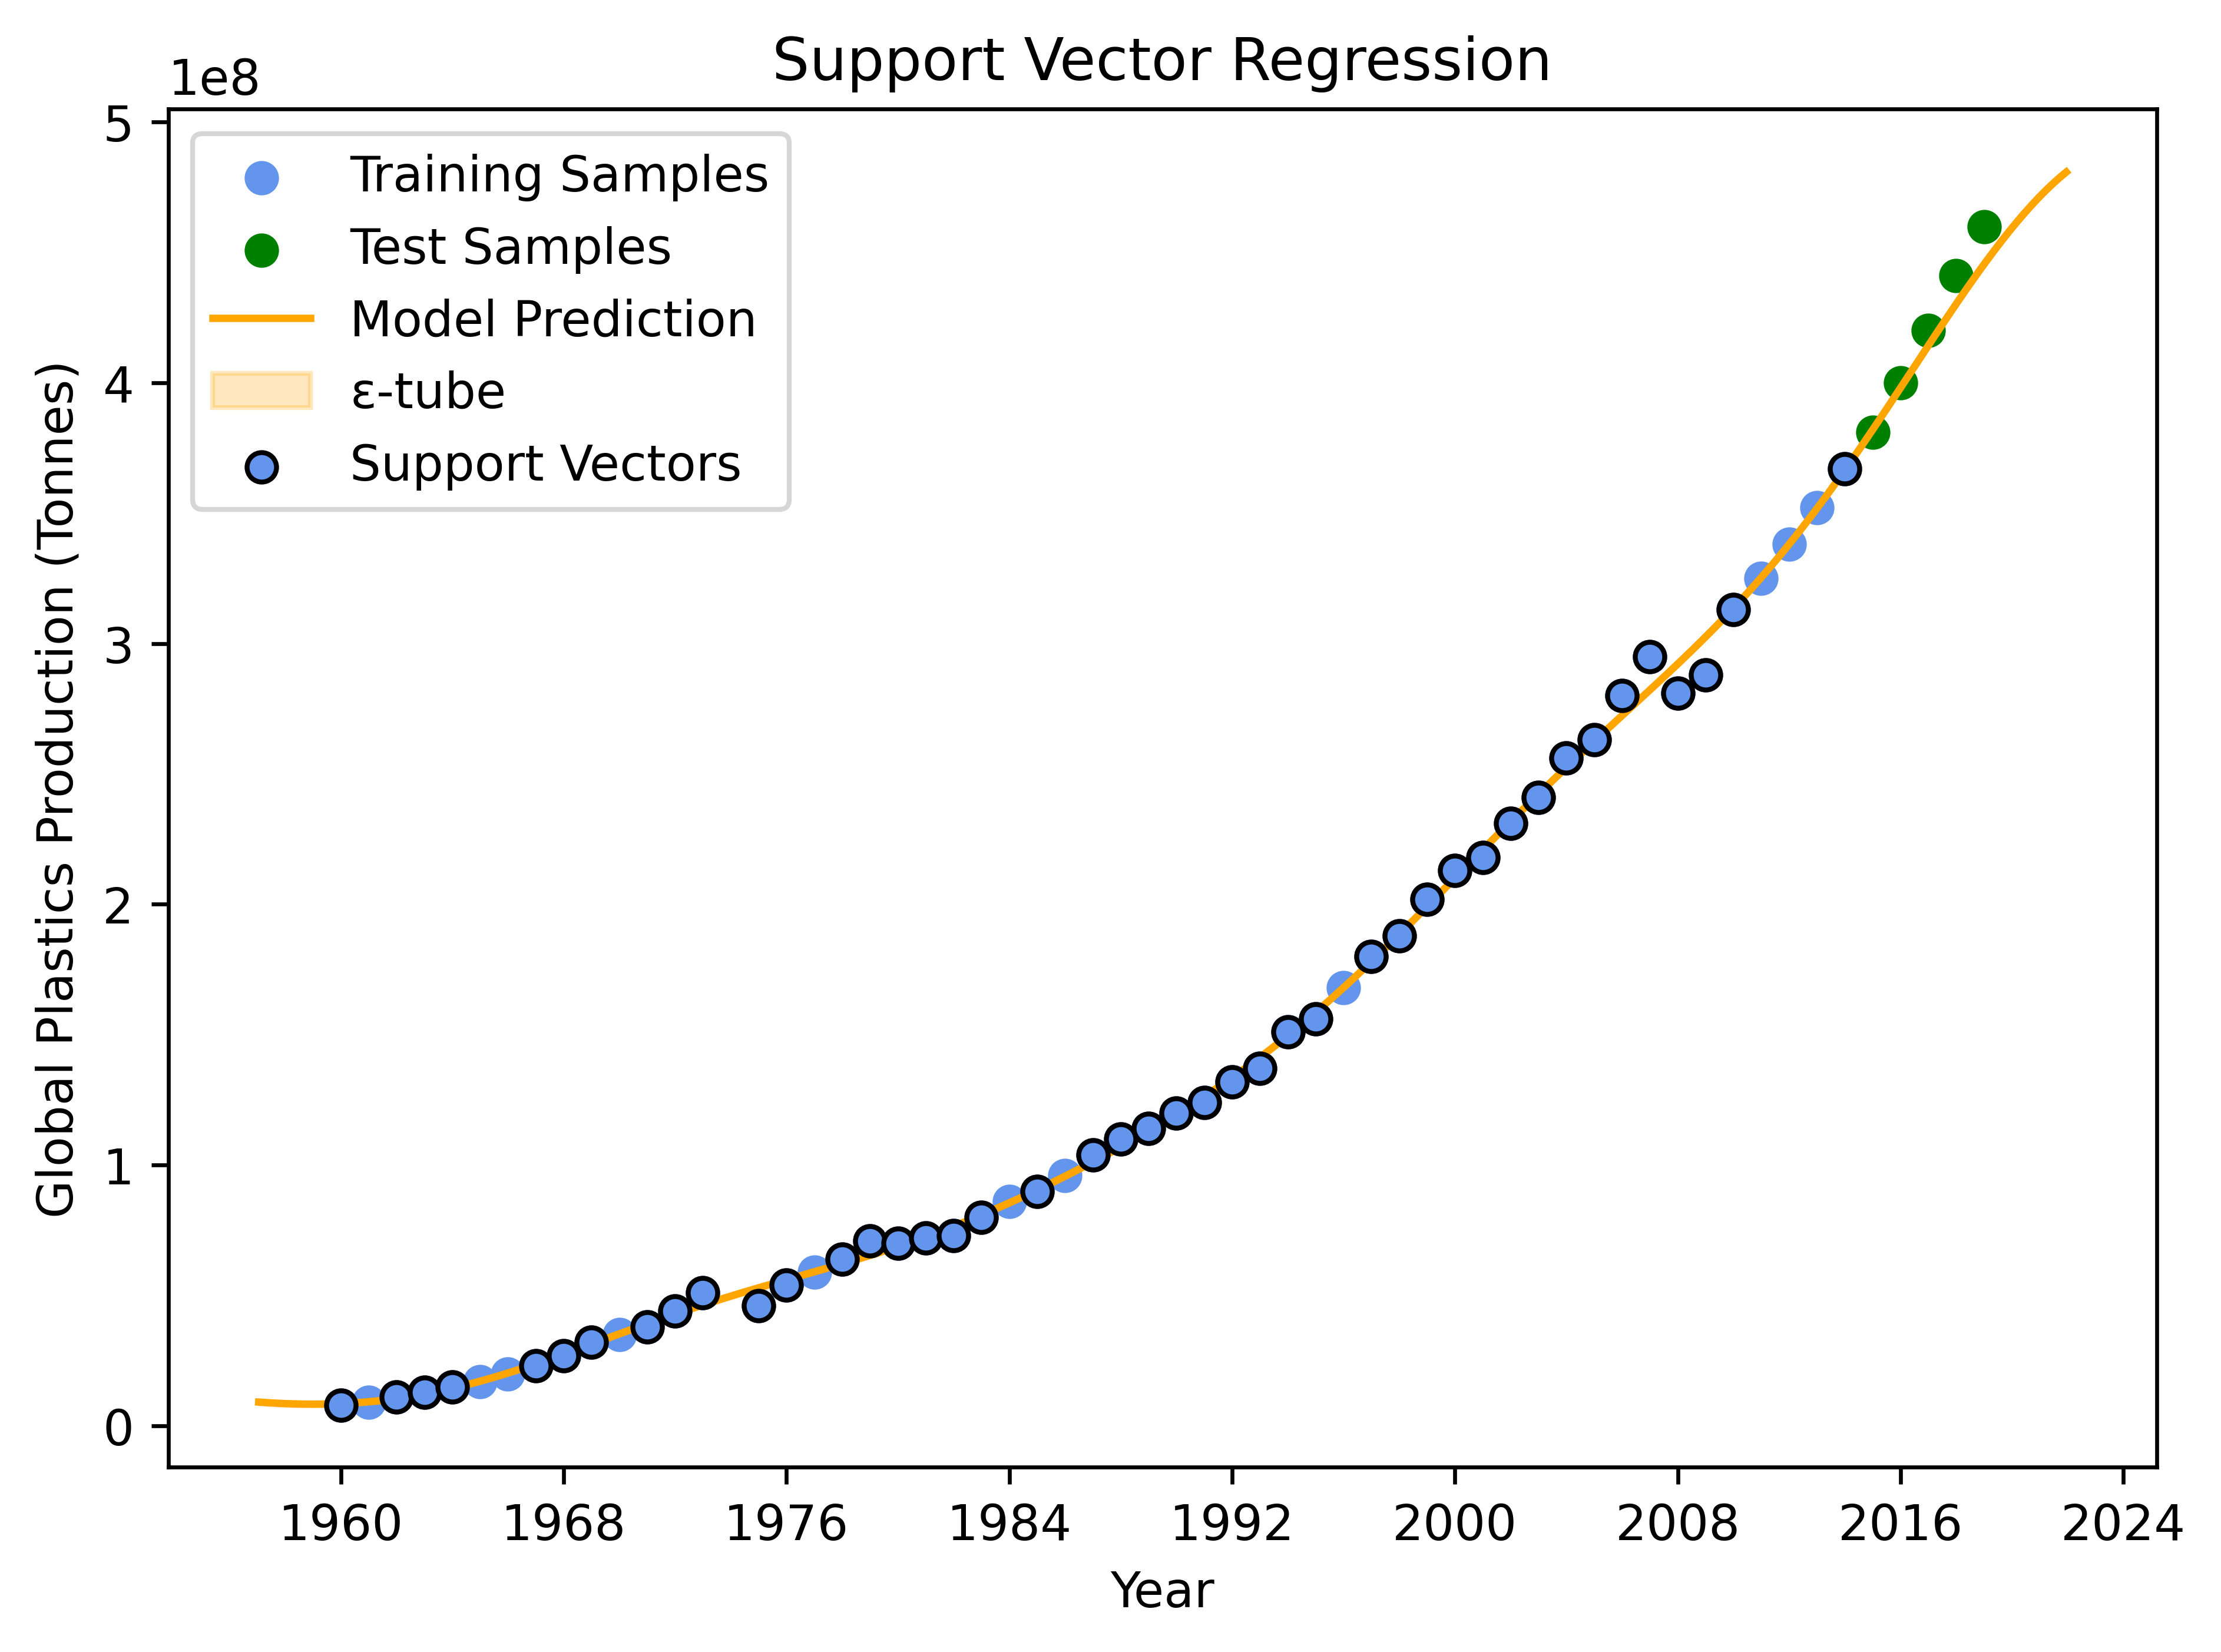
\includegraphics[width=0.45\textwidth]{figures/global_forecasting_svr.png}
	}

	\caption{Forecasts of global plastic production produced by four representative regression models.}
	\label{fig:global_forecasting}
\end{figure}


Figure~\ref{fig:global_forecasting} shows observed values and fitted forecasts for one run of each method across the test windows.
The plotted predictions illustrate individual runs and therefore do not correspond exactly to the average WAPE values reported in Table~\ref{tab:global_forecasting_by_origin}.

% (This tabular data comes from a Linux server, do not edit this)
\begin{table}[!ht]
	\centering
	\caption{
				\centering Hyperparameter tuning time (seconds, rounded to two decimal places) for tunable global plastic production forecasting models under grid search and random search. Time reduction is calculated as \((\text{grid-search time} - \text{random-search time}) / \text{grid-search time}\). The \textsuperscript{*} marker denotes the SVR variant with \(\gamma\) tuning enabled.
		}
		\begin{tabular}{@{}lccc@{}}
			\toprule
			\textbf{Experiment}    & \textbf{Grid Search (s)} & \textbf{Random Search (s)} & \textbf{Time Reduction} \\
			\midrule
			Ridge Regression       & 5.81                     & 3.01                      & 48.15\%                  \\
			SVR                    & 4.65                     & 2.61                      & 43.81\%                  \\
			SVR\textsuperscript{*} & 70.49                    & 2.47                      & 96.49\%                  \\
		\hline
	\end{tabular}
	\label{tab:global_forecasting_tuning_time}
\end{table}


Table~\ref{tab:global_forecasting_grid_search_metrics} and Table~\ref{tab:global_forecasting_random_search_metrics} show that random search evaluated fewer configurations and reduced hyperparameter-tuning time for all tunable models, but its predictive performance was not uniformly equivalent to grid search.
Random search produced lower WAPE for ridge regression, whereas grid search produced lower WAPE for SVR and SVR\textsuperscript{*}.
As shown in Table~\ref{tab:global_forecasting_tuning_time}, random search reduced tuning time by \(48.15\%\) for ridge regression and \(43.81\%\) for SVR.
For SVR\textsuperscript{*}, which tunes three hyperparameters including \(\gamma\), grid search evaluates \(M^3 = 1728\) configurations, where \(M = 12\).
In comparison, random search draws a fixed \(T = 128\) configurations and reduced tuning time by \(96.49\%\).
We therefore use random search in the subsequent case studies as a computational-budget choice, while recognizing that it can yield different predictive performance from grid search.

\subsubsection{Japanese Plastic Waste Generation}

In Experiment 6, we evaluate the same forecasting models on the \texttt{YearPWG (Japan)} dataset.
This series contains only 26 annual observations, and hence the hold-out set is small.

\begin{figure}[H]
	\centering
	\subfloat[Auto ARIMA regression.]{
		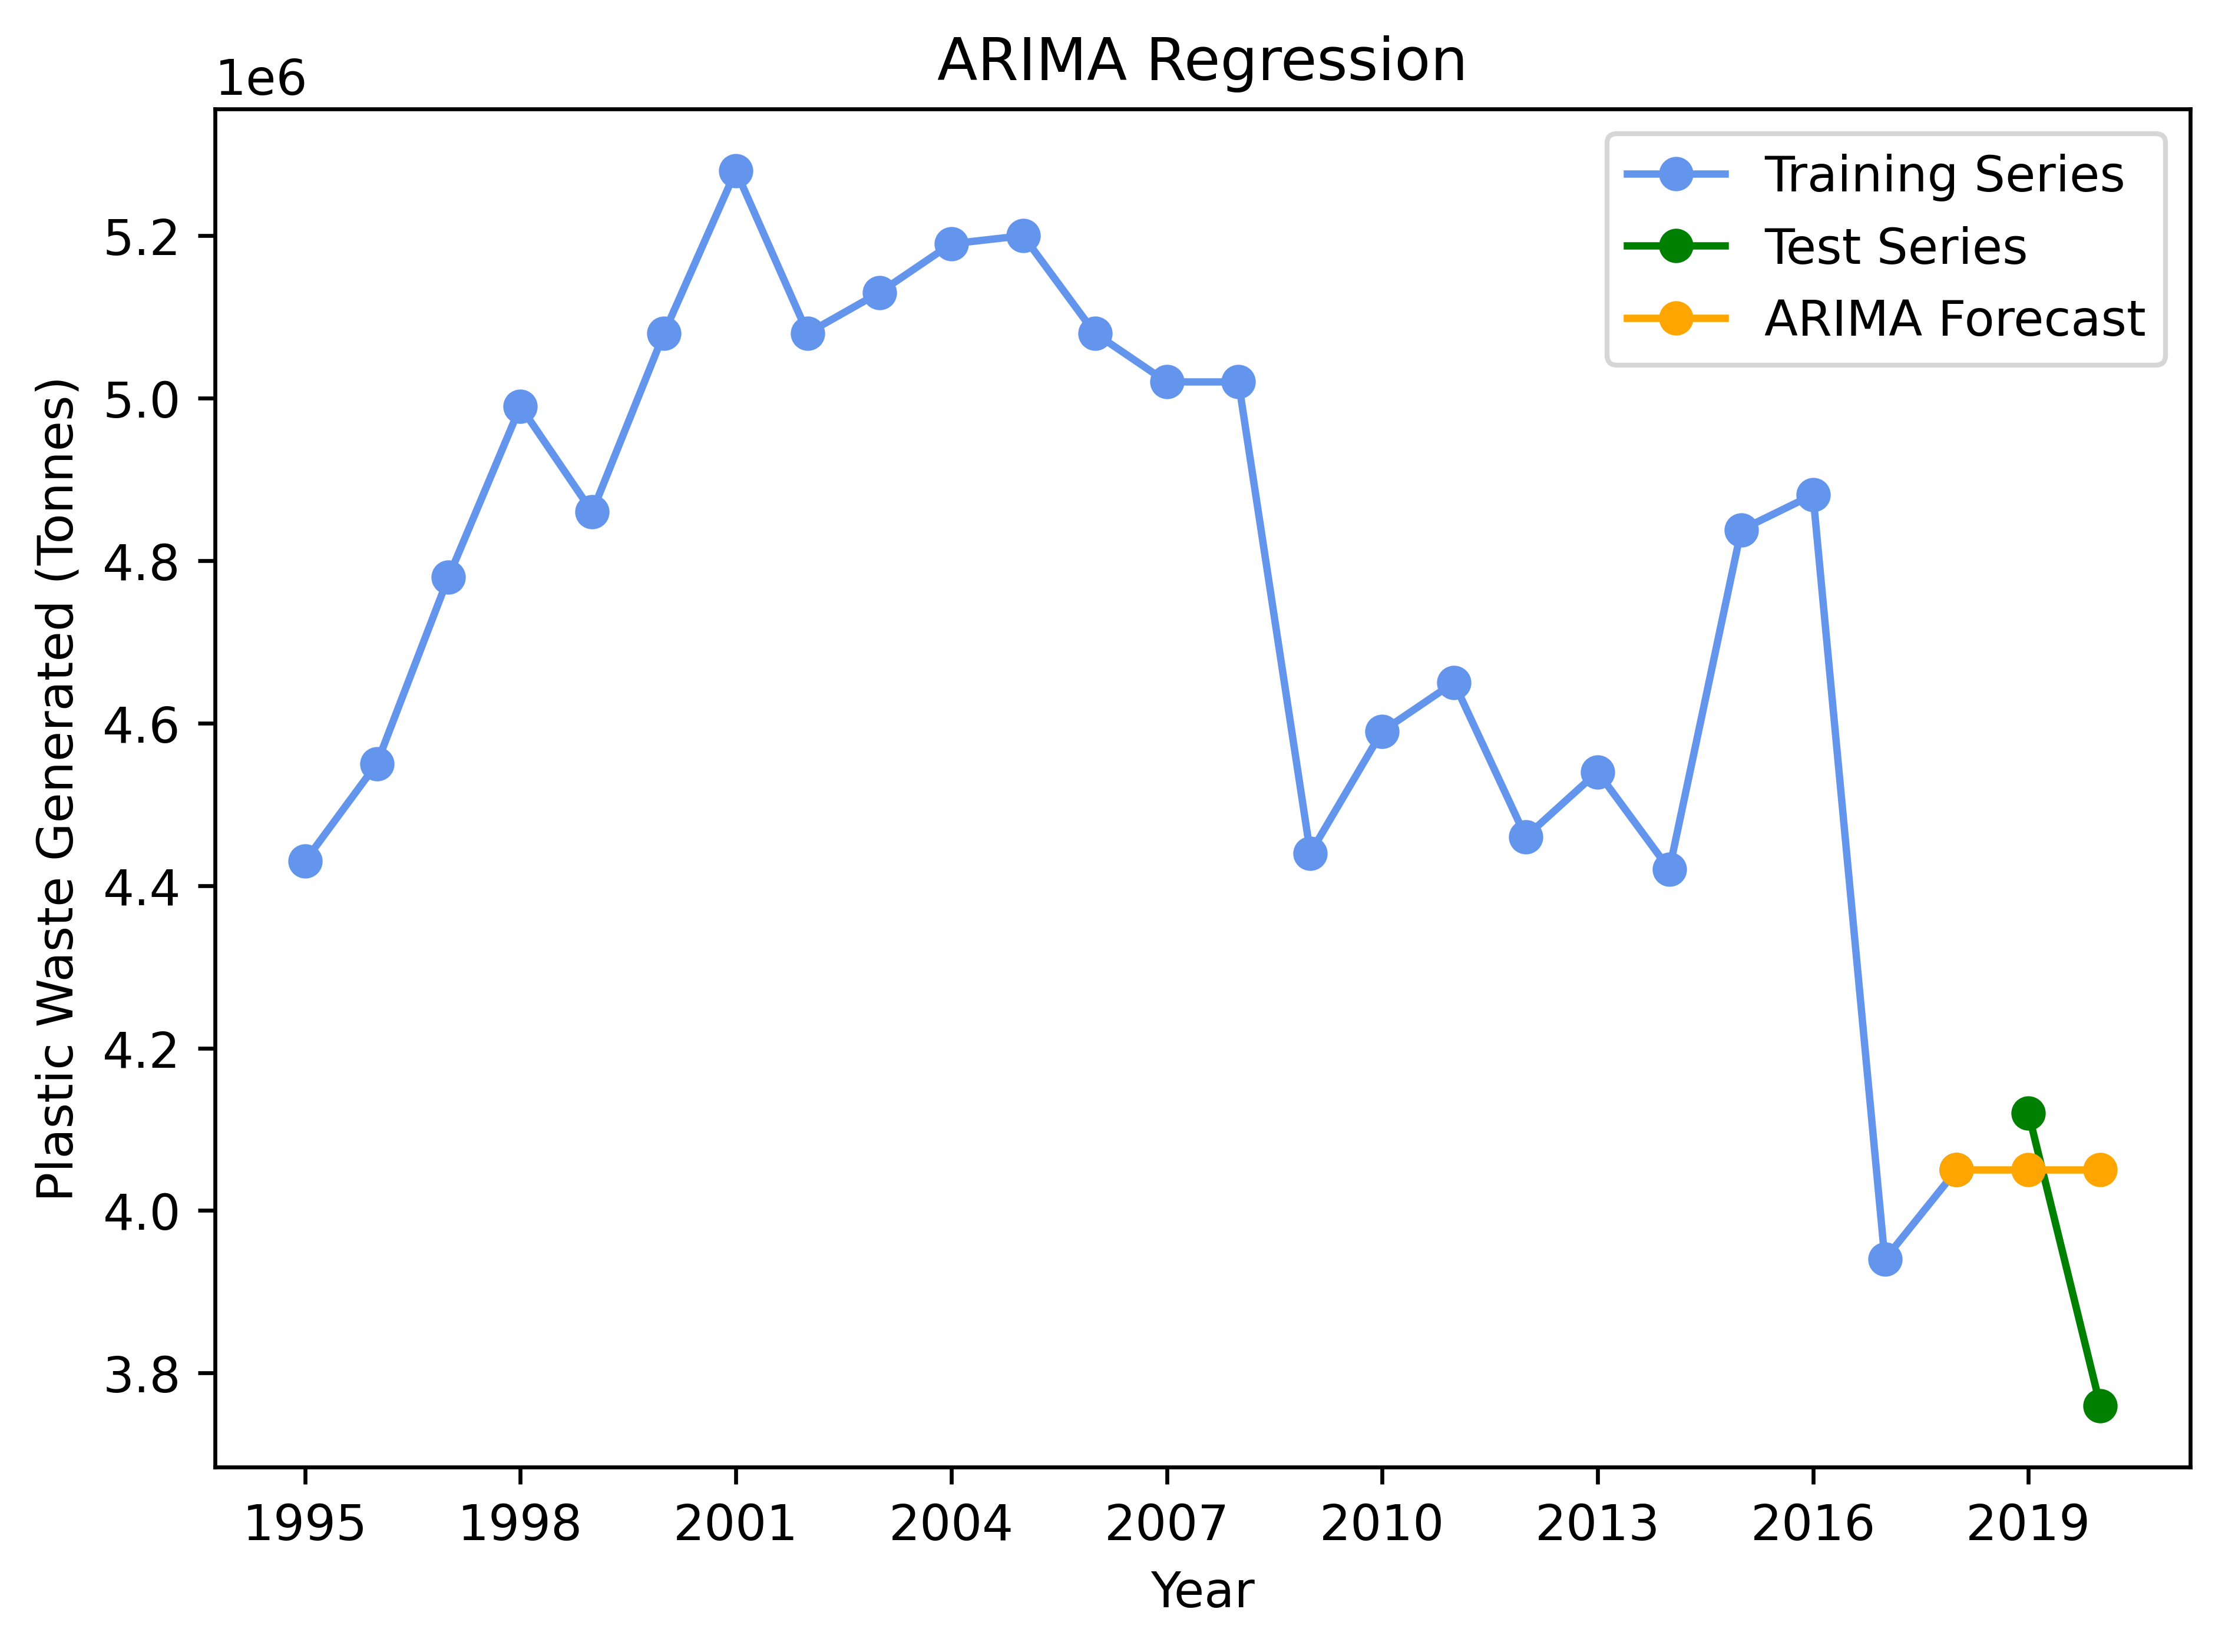
\includegraphics[width=0.45\textwidth]{figures/japan_pwg_forecasting_arima_regression.png}
	}
	\hfill
	\subfloat[Ridge regression.]{
		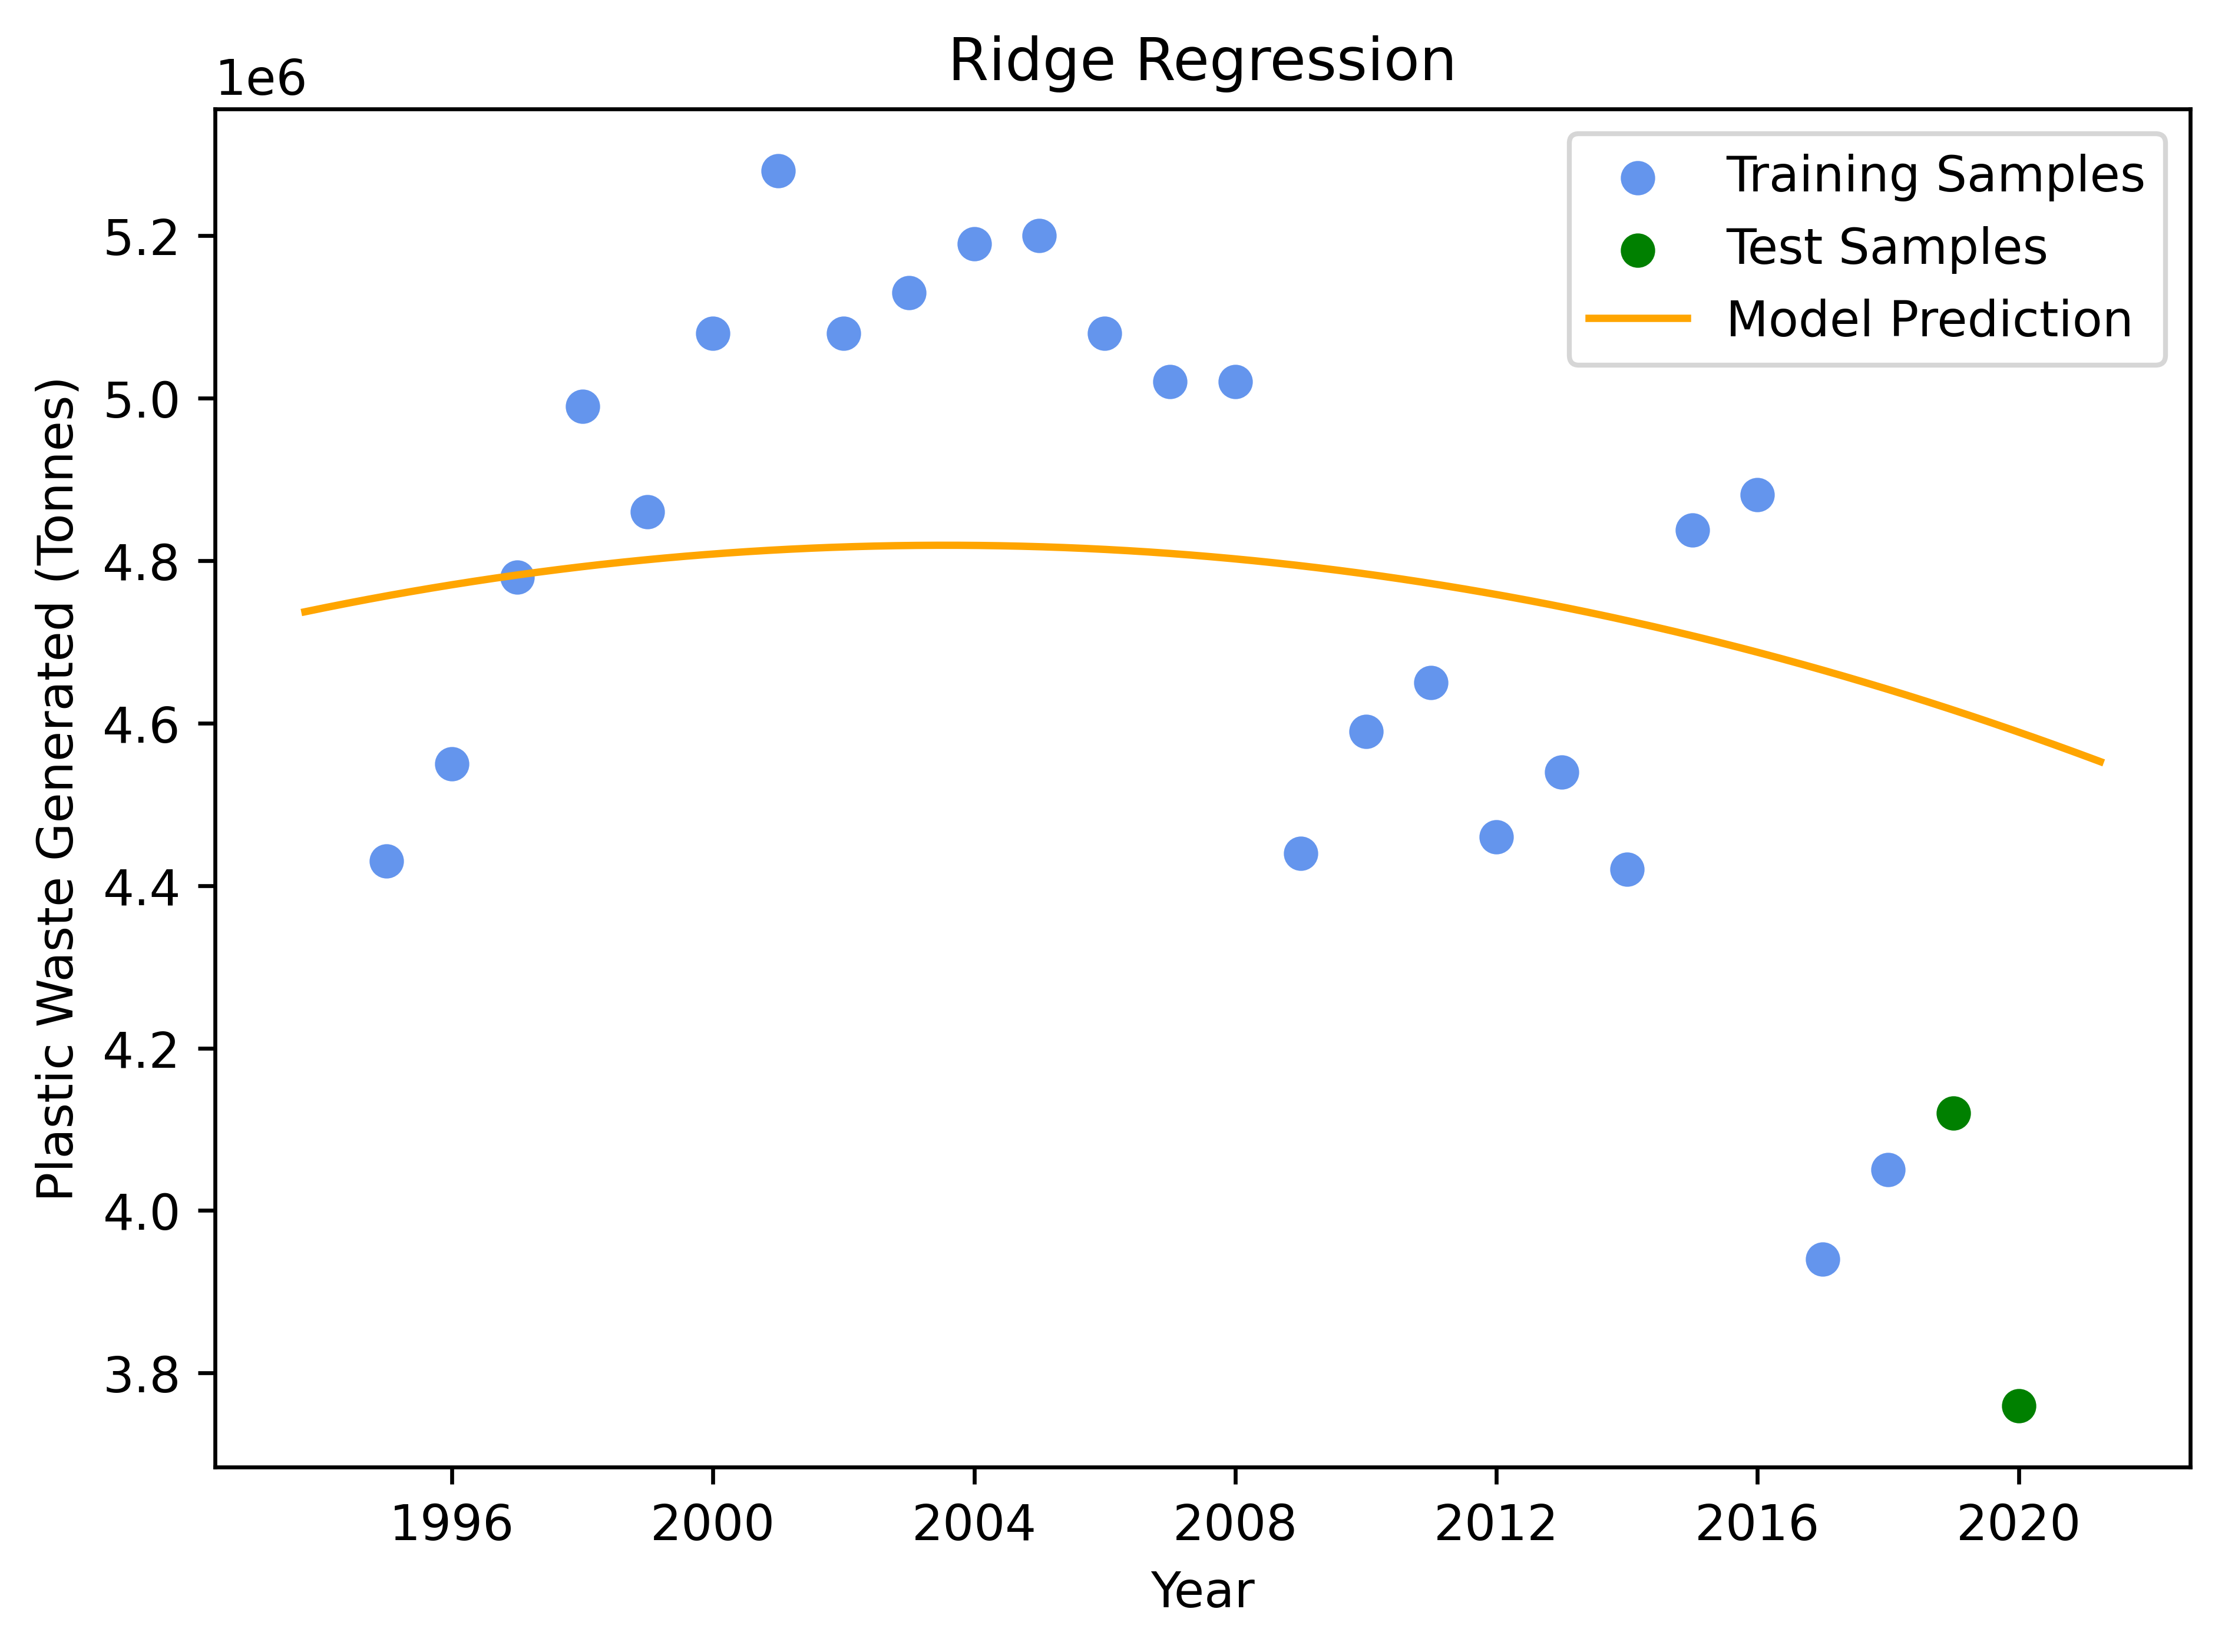
\includegraphics[width=0.45\textwidth]{figures/japan_pwg_forecasting_ridge_regression.png}
	}

	\vspace{0.5cm}

	\subfloat[GPR.]{
		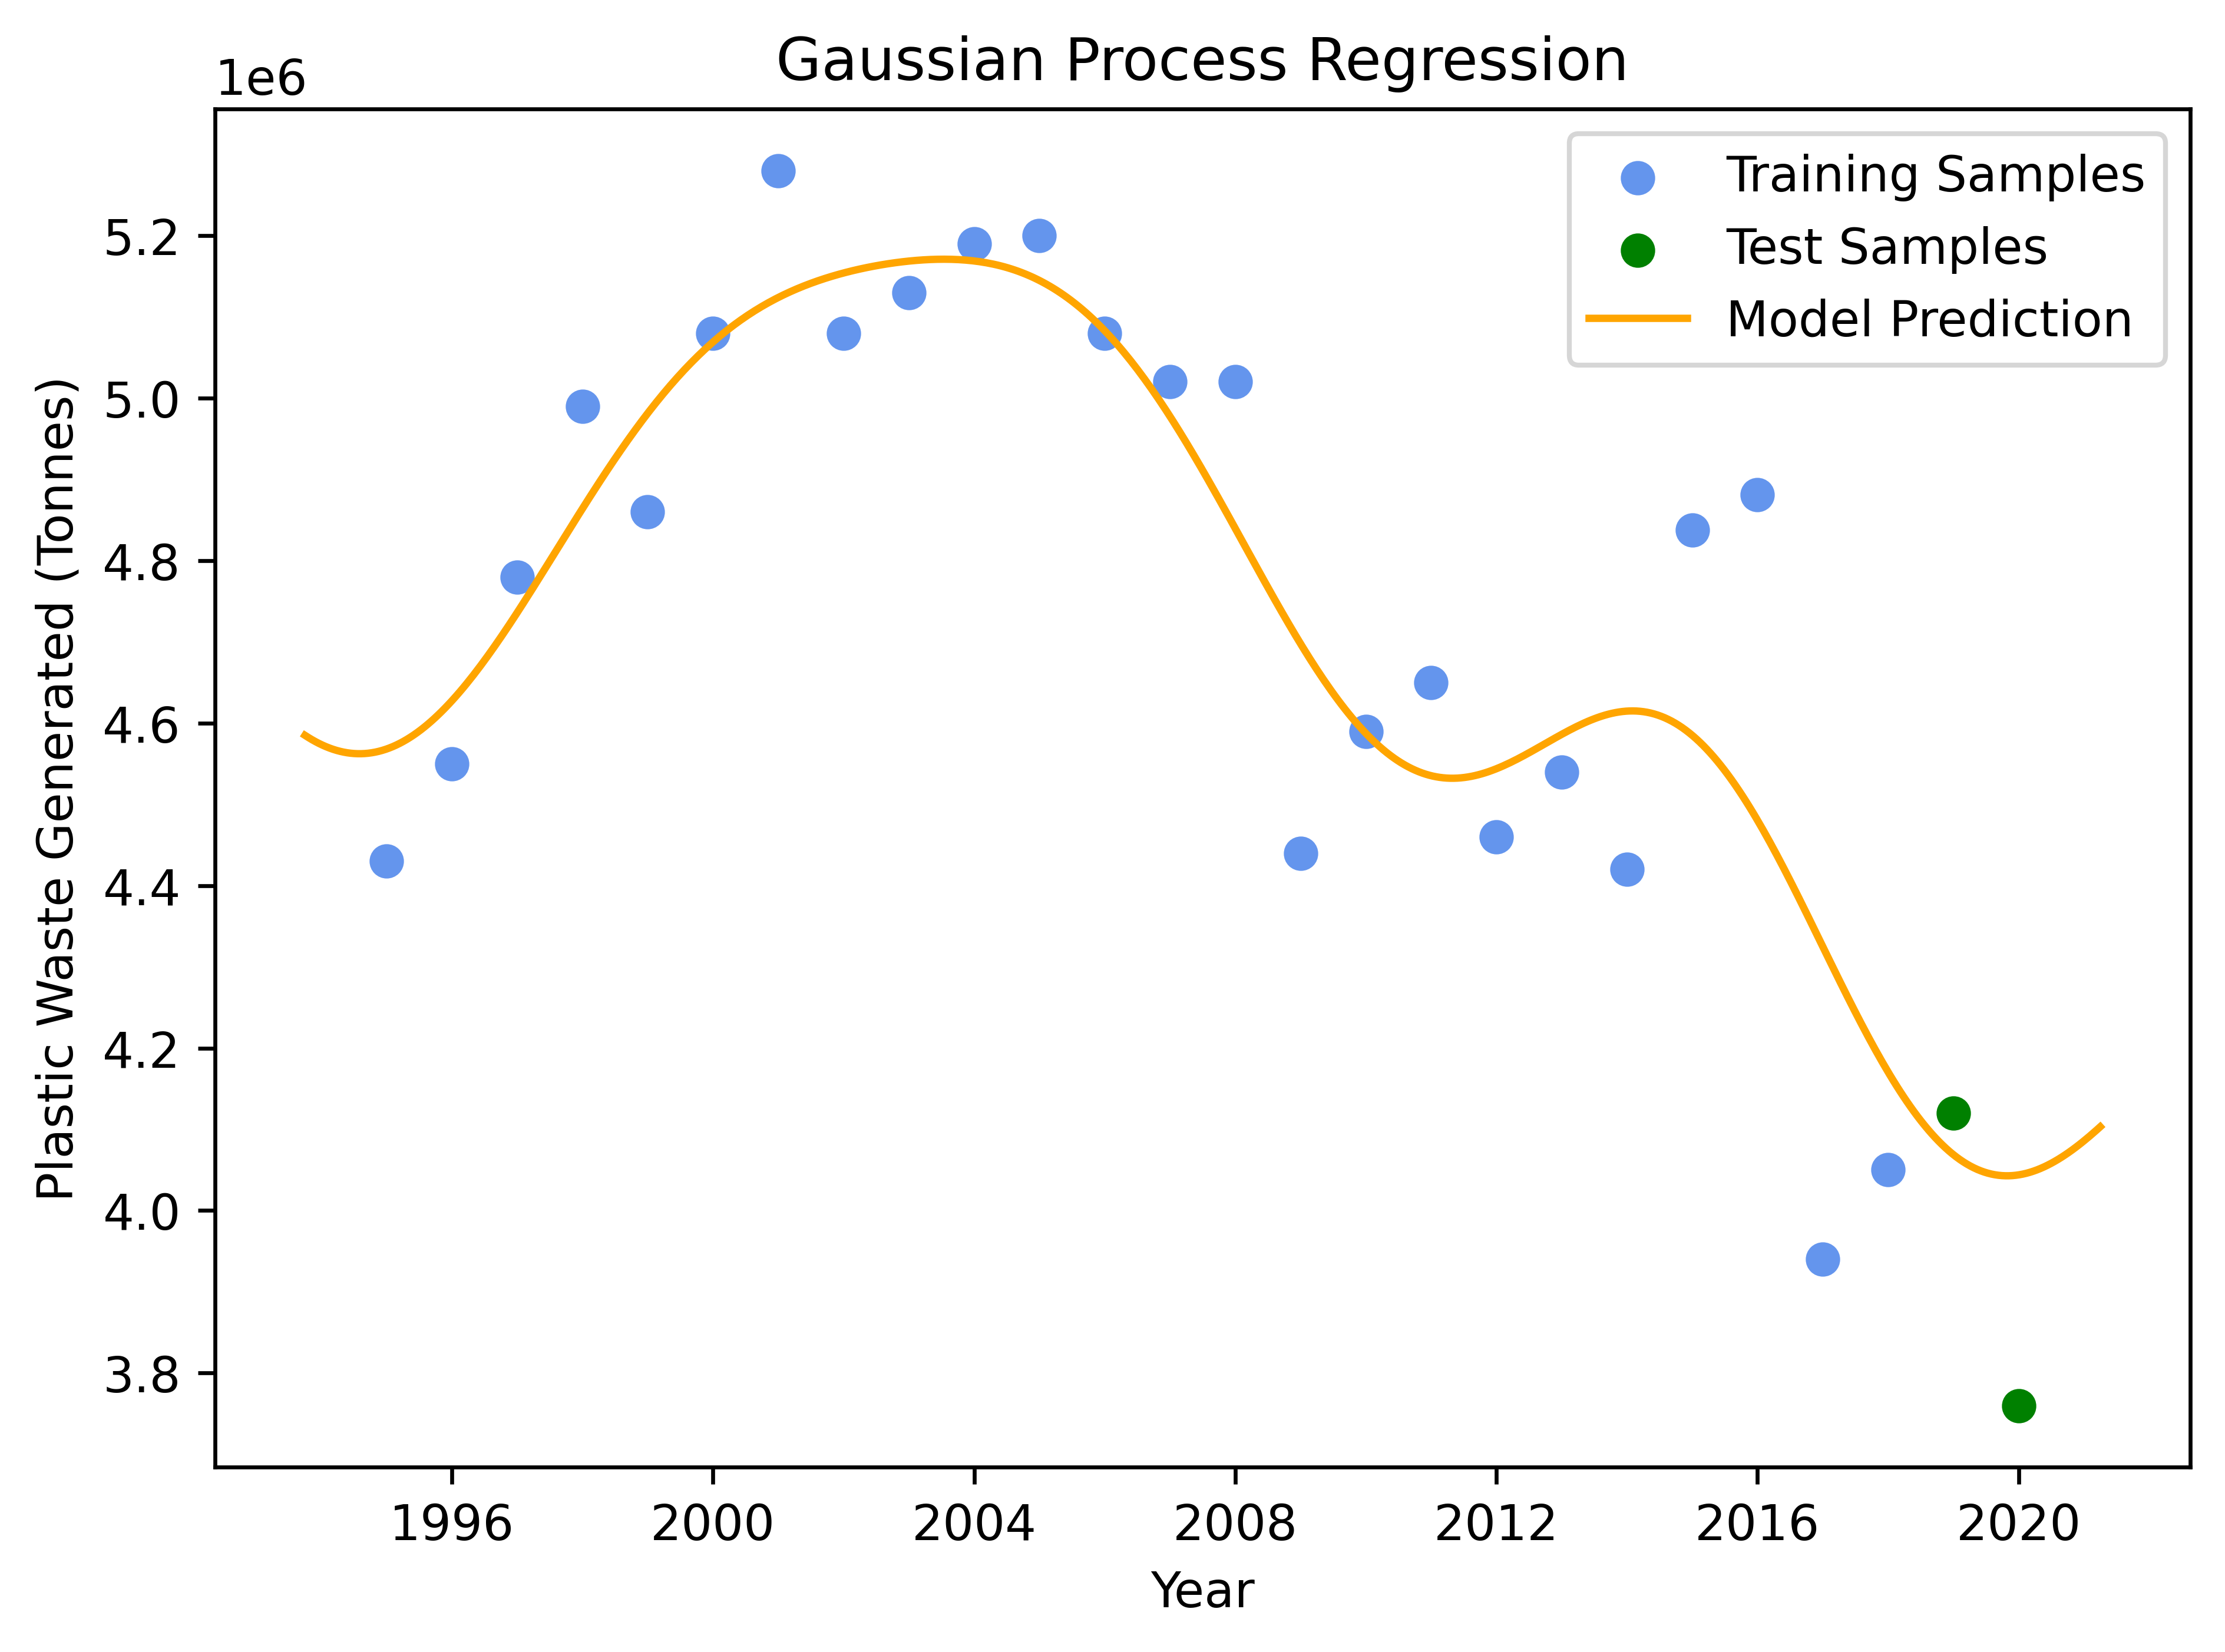
\includegraphics[width=0.45\textwidth]{figures/japan_pwg_forecasting_gpr.png}
	}
	\subfloat[SVR.]{
		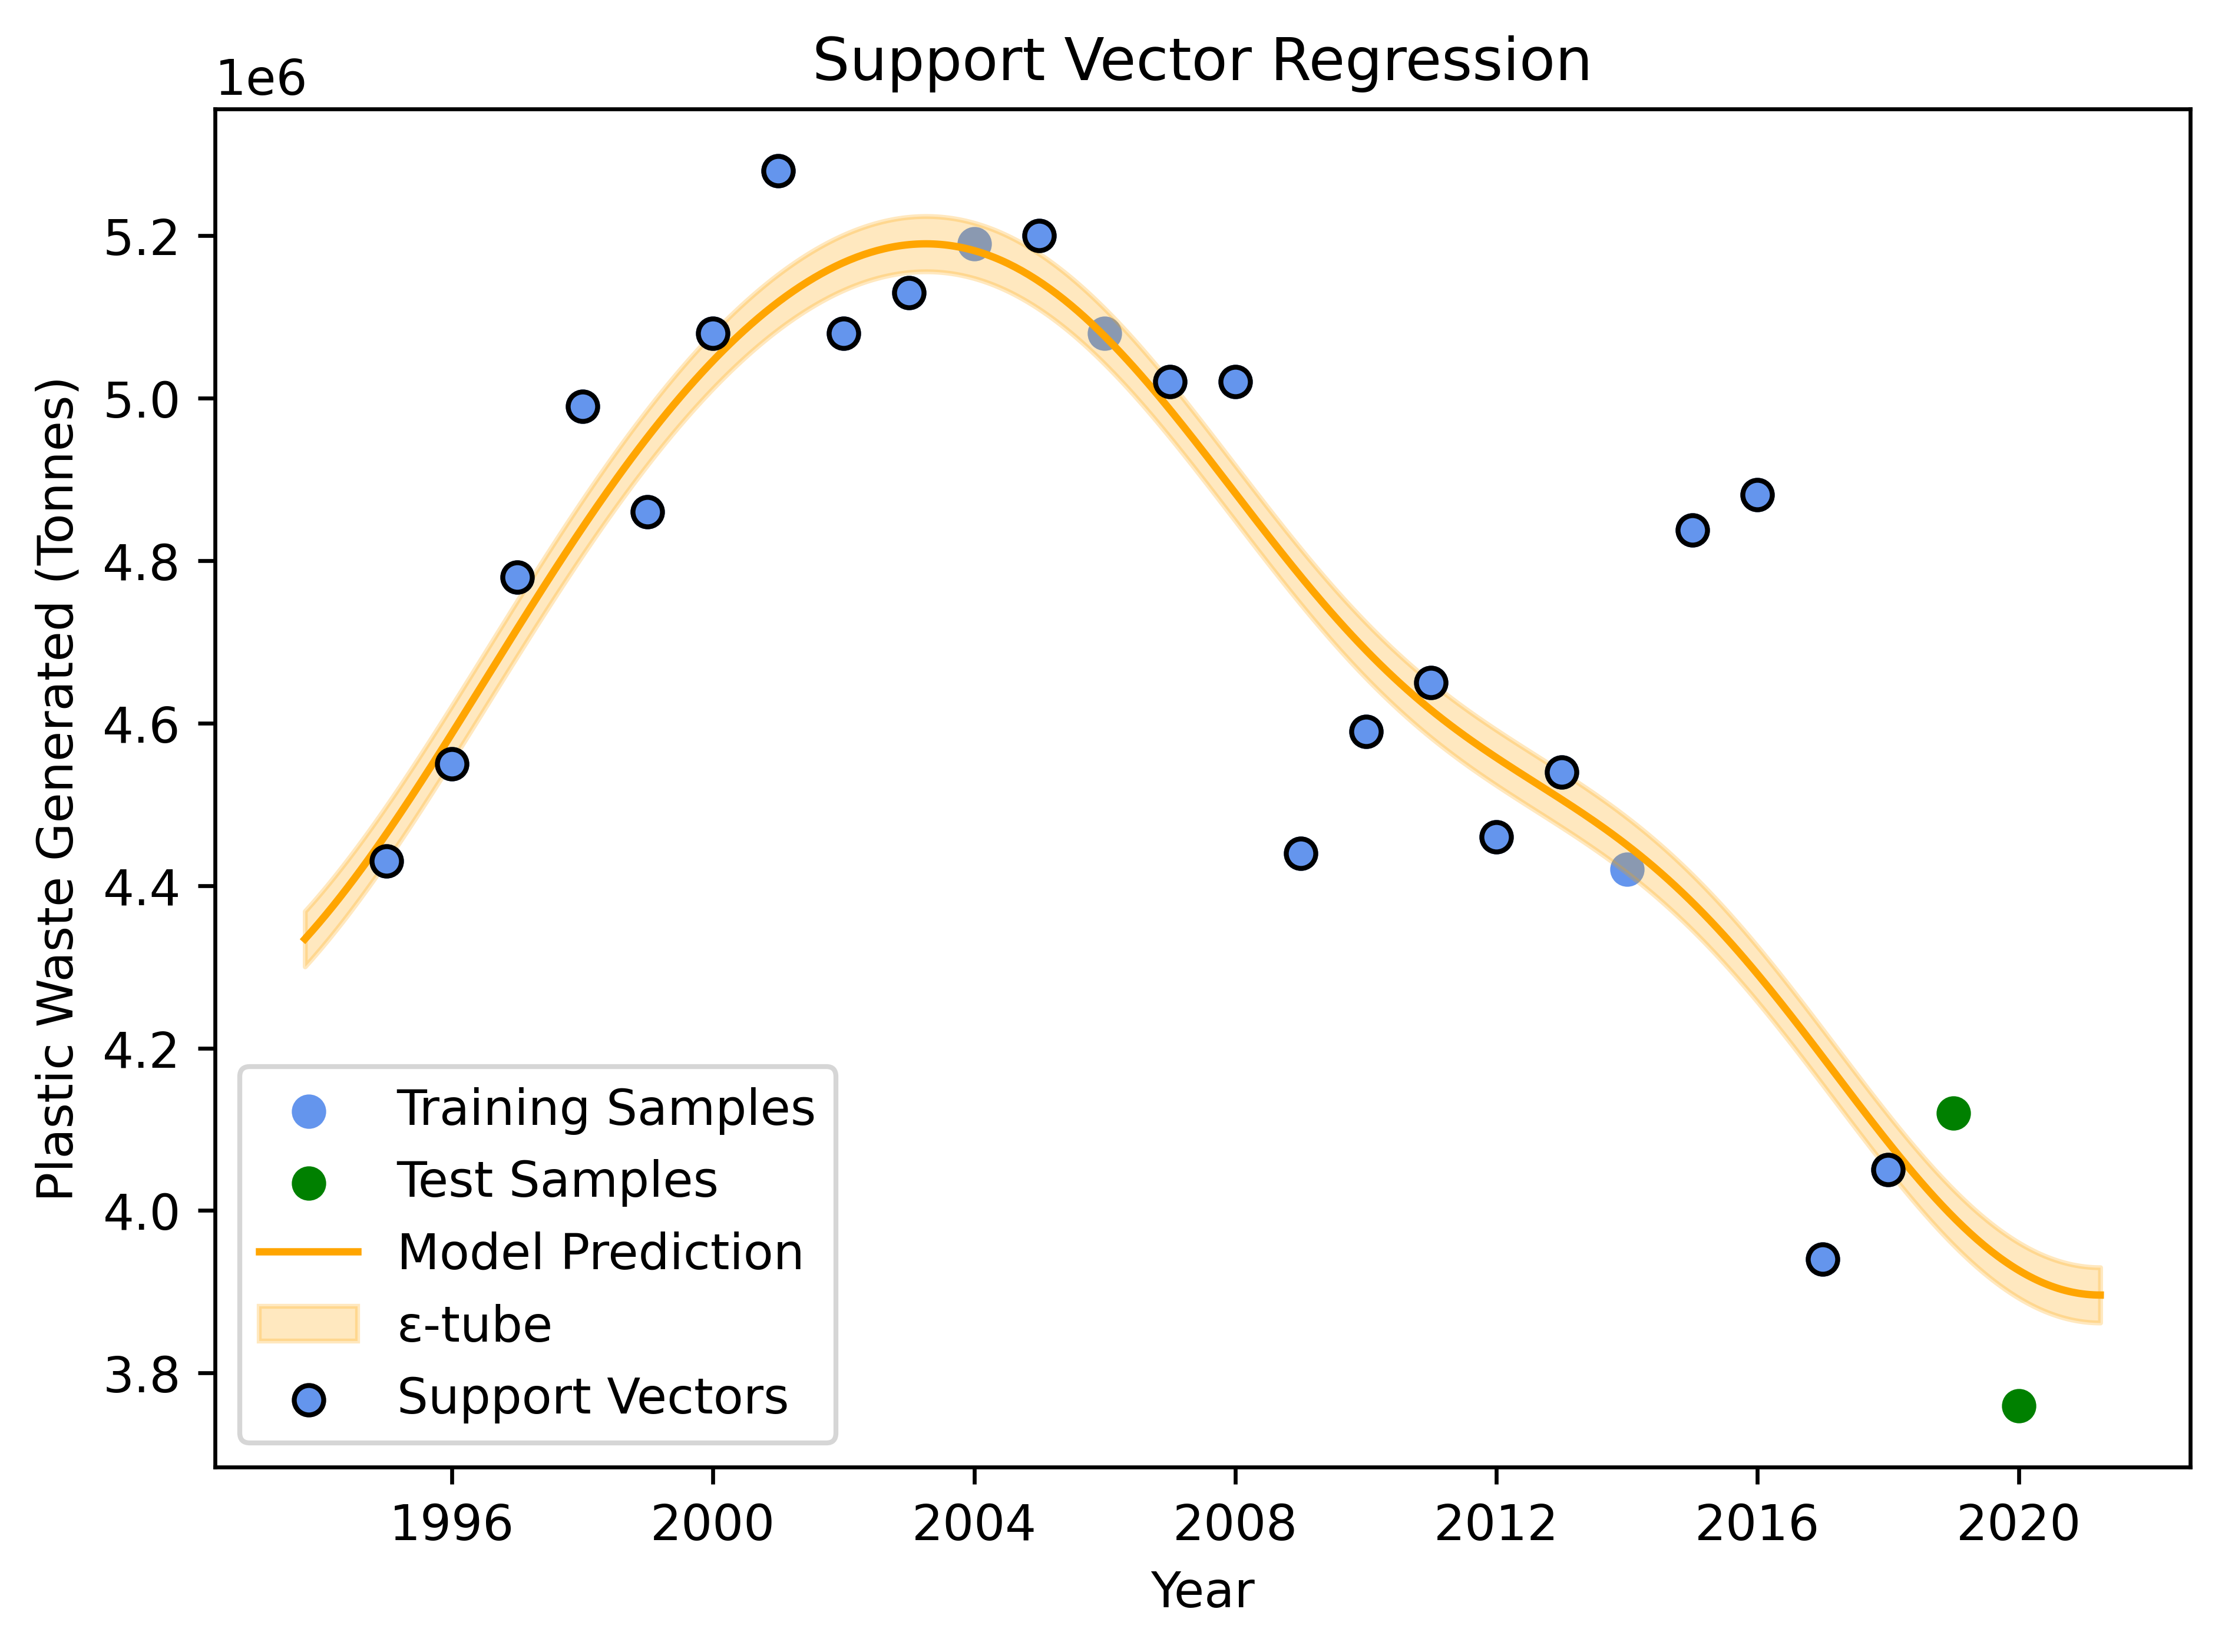
\includegraphics[width=0.45\textwidth]{figures/japan_pwg_forecasting_svr.png}
	}

	\caption{Forecasts of plastic waste generation in Japan by four representative regression models.}
	\label{fig:forecasting_japan_pwg}
\end{figure}

% results/rolling_forecasting_japan/metric_table
\begin{table}[!ht]
	\centering
	\caption{\centering Temporal forecasting performance for plastic waste generation in Japan using the \texttt{YearPWG (Japan)} dataset, averaged first over 16 runs at each origin and then over four forecast origins, with 2 test observations per origin.}
	\begin{tabular}{@{}lccc@{}}
		\toprule
		\textbf{Experiment}    & \textbf{MAE}                   & \textbf{RMSE}                  & \textbf{WAPE}       \\
		\midrule
		\textbf{Naive Persistence} & \(\mathbf{3.914 \times 10^{5}}\) & \(\mathbf{4.005 \times 10^{5}}\) & \textbf{9.28\%} \\
		Drift Baseline & \(3.978 \times 10^{5}\) & \(4.038 \times 10^{5}\) & 9.44\% \\
		Exponential Smoothing & \(4.700 \times 10^{5}\) & \(4.717 \times 10^{5}\) & 11.10\% \\
		Theil--Sen Regression & \(4.487 \times 10^{5}\) & \(4.623 \times 10^{5}\) & 10.53\% \\
		\textbf{ARIMA Regression} & \(\mathbf{3.914 \times 10^{5}}\) & \(\mathbf{4.005 \times 10^{5}}\) & \textbf{9.28\%} \\
		Ridge Regression & \(4.682 \times 10^{5}\) & \(4.772 \times 10^{5}\) & 11.12\% \\
		GPR & \(3.970 \times 10^{5}\) & \(4.139 \times 10^{5}\) & 9.52\% \\
		SVR & \(4.457 \times 10^{5}\) & \(4.519 \times 10^{5}\) & 10.71\% \\
		SVR\textsuperscript{*} & \(5.107 \times 10^{5}\) & \(5.208 \times 10^{5}\) & 11.95\% \\
		\hline
	\end{tabular}
	\label{tab:forecasting_japan_pwg_metrics}
\end{table}

Run-to-run standard deviations for these results are reported in Appendix~\ref{sec:appendix_d}.

Unlike the global plastics production series, the Japan plastic waste generation series is not generally monotonic.
Figure~\ref{fig:forecasting_japan_pwg} shows that the trend increases in the earlier years, declines sharply, and then partially recovers.
This makes the task a useful check of whether flexible regression models can handle short and irregular environmental time series.

Among the three machine learning models, GPR has the lowest WAPE of \(9.52\%\), followed by SVR with a WAPE of \(10.71\%\).
The identical metric values for naive persistence and ARIMA regression are not coincidental.
In this study, ARIMA selected order \((0,1,0)\) with \texttt{trend='n'}, corresponding to a random walk without drift. Therefore, its forecast remains at the last observed value.

Performance differed between the two case studies. Theil--Sen regression had the lowest mean WAPE for global plastic production, while naive persistence and ARIMA had the lowest mean WAPE for Japan’s plastic-waste series.
In these two case studies, none of the evaluated machine-learning models outperformed the best baseline or statistical model by mean WAPE.

Because each evaluation uses a short series and a limited number of forecast origins, the rankings should be interpreted cautiously.
